\chapter{Audioa eta bideoa}\index{<video>}
\index{<audio>}\index{HTMLMediaElement}

HTML5 estandarrak <video> eta <audio> etiketak sartu zituen, eta horiekin batera, JavaScript bidez audioa eta bideoa kontrolatzeko HTMLMediaElement APIa. Bideoarekin lan egiten hasiko gara, termino batzuk definituz, \textit{kontainer}, \textit{codec} eta formatuak, besteak beste. 


\begin{figure}[ht]
	\centering
\begin{tikzpicture}
\node[anchor=south west,inner sep=0] (image) at (0,0)
   {\includegraphics[trim=0cm 0cm 0cm 0cm, clip=true, width=0.75\textwidth]{img/native-controls-firefox.png}};
\end{tikzpicture}
\caption{Audio —goian— eta bideo —behean— kontrol-osagaiak.}
\label{fig:bideocontrols}
\end{figure}

\section{\textit{Kontainer} eta \textit{codec}-ak}\index{kontainer}\index{codec}
Bideo-fitxategi baten inguruan hitz egitean askotan entzun izan ditugu ``AVI fitxategi'' edo ``MP4 fitxategi'' hitzak. Baina AVI edo MP4 ez dira fitxategi mota bat, baizik eta kontainer motak. AVI MP4\index{MP4} edo WebM \index{WebM} kontainer batek, bere barnean, audio- eta bideo-kanalak gordetzen ditu, hainbat formatutan kodetuta egon daitezkeenak (\textit{codec} —kodek— ezberdinekin, Theora, H.264, VP9...).

\section{<video> etiketa}

Berez, bideo bat bistaratzeko etiketa sinple bat erabili ahal dugu:

\begin{verbatim}
    <video src="bideoa.webm"></video>
\end{verbatim}

Berriro, WebM kontainer mota bat da. Barruan duen bideoaren formatua (erabili den kodeka) zein den ez dakigu (bideoa jaitsi eta aztertu arte). HTML5 estandarrak \textit{<video>} etiketa eskaintzen badu ere, ez du zehazten bideoak erabili behar duen formatua... edo nabigatzaileak berak onartu behar dituen formatuak. Izan ere, hainbat aukera ditugu (\ref{fig:bideokodek} irudian adibide batzuk zehazten dira).

\begin{figure}[ht]
	\centering
\begin{tikzpicture}
\node[anchor=south west,inner sep=0] (image) at (0,0)
   {\includegraphics[trim=0cm 0cm 0cm 0cm, clip=true, width=0.75\textwidth]{img/bideoformatuak.png}};
\end{tikzpicture}
\caption{Bideo-kontainer eta \textit{codec}-en artean hainbat aukera ditugu.}
\label{fig:bideokodek}
\end{figure}

Nabigatzaile bakoitzak kodek zehatz bat onartzen duen edo ez jakiteko, Wikipediak eskaintzen duen \href{https://en.wikipedia.org/wiki/HTML5_video}{taulara joko dugu}\footnote{https://en.wikipedia.org/wiki/HTML5\_video} (ikus \ref{fig:bideokodekwikipedia}. irudia). Bertan kontainer eta kodeken bateragarritasuna nabigatzailearen arabera zehazten da.



\begin{figure}[ht]
	\centering
\begin{tikzpicture}
\node[anchor=south west,inner sep=0] (image) at (0,0)
   {\includegraphics[trim=0cm 0cm 0cm 0cm, clip=true, width=0.75\textwidth]{img/kodekwikipedia.png}};
\end{tikzpicture}
\caption{Wikipediak badu orri bat nabigatzaileen arteko bideo-kodek eta kontainerren bateragarritasuna neurtzeko.}
\label{fig:bideokodekwikipedia}
\end{figure}


Hori guztia kontuan hartuta, ulertzekoa da <video> etiketaren erabilera aurkeztu dugun adibidea baino konplexuagoa izatea. Hurrengo listatuan <video> etiketaren erabileraren adibide zehatza ikus dezakegu:

\begin{lstlisting}[language=JavaScript,label={lst:bideoadibidea}]
<video width="320" height="240" controls>
 <source src="clip.mp4" type="video/mp4; codecs=avc1,mp4a">
 <source src="clip.webm" type="video/webm; codecs=vp8,vorbis">
 <source src="clip.ogv" type="video/ogg; codecs=theora,vorbis">
</video>
\end{lstlisting}

Bertan 320 x 240 tamainako bideo bat bistaratu nahi dugula zehaztu dugu. Bideoarekin batera, \textit{controls} atributuarekin, \textit{Play}, \textit{Pause}, \textit{FastForward} eta \textit{Rewind} egiteko aukera izan nahi dugula esaten ari gara.\index{<video> controls}

Horrez gain, \hl{type=video/mp4} atributuarekin, MP4 kontainerra hobesten dugula esaten ari gara, barruan avc1 bideo-kodeka eta mp4 audio-kodeka izango dituena (\hl{codecs=avc1,mp4a}). Hori ezinezkoa balitz (nabigatzaileak onartuko ez balu), orduan WebM kontainerra aukeratuko genuke, vp8 \index{VP8} bideo-kodek eta vorbis\index{Vorbis} audioarekin. Eta hori ere ezinezkoa balitz, orduan Ogg \index{OGG} kontainerra izango litzateke gure aukera, \textit{theora video} eta \textit{vorbis} audioarekin.

\textit{Controls} izeneko atributua ez da erabil dezakegun bakarra. Badugu autoplay\index{autoplay}, loop\index{loop}, preload\index{preload} eta poster\index{poster} izenekoak ere.

\begin{itemize}
    \item \textit{autoplay}: bideoa kargatu bezain pronto martxan jarri nahi dugula zehazten du.
    \item \textit{loop}: bideoa amaitzean berriro hasieratik automatikoki hasiko dela adierazteko.
    \item \textit{preload}: \hl{preload=auto} edo \hl{preload=metadata} izan daiteke atributu honen balioa. \textit{Auto}-ren kasuan, nabigatzaileari bideoa ahal bezain pronto kargatzea (orria kargatzen den unean) gomendatzen diogu. Alegia, erabiltzaileak \textit{play} botoian sakatu baino lehen, automatikoki buffer batean bideoa kargatzea nahi dugula zehazten du. Horrela erabiltzaileak \textit{play} botoian sakatzean, bideoa berehala hasiko da bistaratzen, inolako etenik gabe. \textit{Metadata}-ren kasuan gauza bera, baina bideo osoa aurrekargatu beharrean, bideoaren metadatuak (luzera, \textit{track} kopurua, bideoaren lehenengo fotograma, poster gisa erabiltzeko...) aurrekargatuko dira
   \item \textit{poster}: bideoa hasi baino lehen pantailan bideoari dagokion irudi txiki bat agertuko da.
\end{itemize}

Bideo bat JS erabiliz kontrolatzeko API bat daukagu eskuragarri HTML5en. Metodo, atributu eta gertaera asko eskaintzen baditu ere, garrantzitsuenak \ref{tab:bideoAPI}. taulan aurki daitezke.

% Please add the following required packages to your document preamble:
% \usepackage{booktabs}
\begin{table}[]
\begin{tabular}{@{}lllll@{}}
\toprule
\multicolumn{2}{c}{\textbf{Atributuak}} & \multicolumn{1}{c}{\textbf{Metodoak}} & \multicolumn{2}{c}{\textbf{Gertaerak}} \\ \midrule
width            & currentTime          & play()   \index{play()}                             & progress            & timeupdate       \\
height           & paused               & pause()   \index{pause()}                            & loadeddata          & volumechange     \\
loop             & duration             & load() \index{load()}                               & error               & ended            \\
muted            & readyState           & canPlayType()   \index{canPlayType()}                       & loadedmetadata      & play            \\
ended            & seeking              &                                       & pause               & abort            \\
error            & volume               &                                       & waiting             &                  \\ \bottomrule
\end{tabular}
\caption{Bideoak JavaScript-ez kontrola ditzakegu, hainbat metodo, atributu eta gertaeraren bidez.}
\label{tab:bideoAPI}
\end{table}

Bideoen inguruko APIa hobeto ulertzeko adibide pare bat ekarriko ditugu hona. Lehenengoak hiru bideo kargatzen ditu array batean eta, APIa erabiliz, bata bestearen ondoren joko ditu. 

\begin{lstlisting}[language=JavaScript]
let position = -1;
let playlist;
let bideo;
window.onload = function() {
	playlist = ["video/bat.mp4","video/bi.mp4", "video/hiru.mp4"];
	bideo = document.getElementById("video");
	bideo.addEventListener("ended", hurrengoBideoa);
        hurrengoBideoa();
}

function hurrengoBideoa(){
     position++;
     if (position >=  playlist.length) position = 0;
     bideo.src = playlist[position];
     bideo.load();
     bideo.play();
}
\end{lstlisting}


Bigarren adibidean gauza bera egiten dugu, baina bideoa martxan jarri baino lehen bideoaren kontainerra nabigatzaileak onartzen duen edo ez begiratuko dugu. 

\begin{lstlisting}[language=JavaScript]

window.onload = function() {
// ...
	playlist = ["video/bat","video/bi", "video/hiru"];
// ...
}
function hurrengoBideoa(){
// ...
     bideo.src = playlist[position] + getFormatExtension();
// ...
}
function getFormatExtension() {
    if (bideo.canPlayType("video/mp4") != "") {
    	    return ".mp4";
    } else if (bideo.canPlayType("video/ogg") != "") {
        return ".ogv";
    } else if (bideo.canPlayType("video/webm") != "") {
        return ".webm";
    }
}
\end{lstlisting}


 \begin{alertinfo}{canPlayType() metodoaren balio posibleak}
        Bideoa baten \textit{canPlayType()}\index{canPlayType()} metodoak parametro bat hartzen du, bideoaren kontainer mota (adibidez "video/webm", edo "video/mp4") eta hiru balio posible itzultzen ditu: kate hutsa (""), "maybe" edo "probably". Kate hutsaren kasuan, nabigatzaileak kontainer mota hori ez duela onartzen esan nahi du. \textit{maybe} kasuan, agian bistaratu dezakeela eta \textit{probably} ia ziur onartzen duela. Nabigatzaileak ezin du erabat ziurtatu jo ahal duen edo ez, kontainer baten barruan kodek ezberdinak egon daitezkeelako.
    \end{alertinfo}

\section{Audio-etiketa}\index{<audio>}

Audioaren eta bideoaren etiketek oso antzera funtzionatzen dute. Ikus bestela honako HTML5 <audio> etiketaren adibidea:

\begin{lstlisting}[language=JavaScript]
<audio controls>
<source src="horse.ogg" type="audio/ogg">
<source src="horse.mp3" type="audio/mpeg">
Zure nabigatzaileak ez du audio etiketa onartzen.
</audio>
\end{lstlisting}

Ogg motako kontainerra ez bada onartzen, orduan MP3 kontainer mota duen audioarekin saiatuko gara. Horrekin ere ezin badu nabigatzaileak, orduan errore-mezu bat emango dugu. Ohart zaitez \textit{controls} atributua ere erabiltzen ari garela (ikus \ref{fig:audiocontrols}. irudia).

\begin{figure}[ht]
	\centering
\begin{tikzpicture}
\node[anchor=south west,inner sep=0] (image) at (0,0)
   {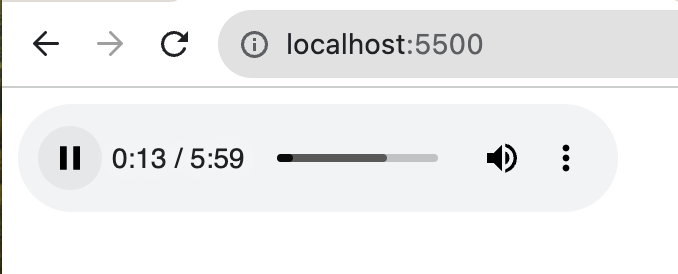
\includegraphics[trim=0cm 0cm 0cm 0cm, clip=true, width=0.75\textwidth]{img/audiobideo/audiocontrols.png}};
\end{tikzpicture}
\caption{Audio player-a, hainbat kontrolekin.}
\label{fig:audiocontrols}
\end{figure}


Nabigatzaileek audio-formatuekin duten bateragarritasun-maila jakin ahal izateko badugu Wikipedian orri berezi bat ere\footnote{\href{http://en.wikipedia.org/wiki/HTML5\_Audio}{http://en.wikipedia.org/wiki/HTML5\_Audio}}.

\section{Ariketak}

Ariketa multzo honetan canvas eta <video> etiketak uztartuko ditugu, adibidez \ref{fig:bideoariketa}. irudian dagoen ariketa egiteko. 

\begin{figure}[ht]
	\centering
\begin{tikzpicture}
\node[anchor=south west,inner sep=0] (image) at (0,0)
   {\includegraphics[trim=0cm 0cm 0cm 0cm, clip=true, width=0.75\textwidth]{img/azala.png}};
\end{tikzpicture}
\caption{Bideo batetik fotogramak atera daitezke eta canvas batean utzi baino lehen itxuraz aldatu. Adibidez, irudia zuri-beltz bihurtzeko.}
\label{fig:bideoariketa}
\end{figure}

Hemengo kode-adibideari jarraituz
\href{https://codesandbox.io/s/bideo-ariketa-1-bh3cg}{https://codesandbox.io/s/bideo-ariketa-1-bh3cg}:

\begin{enumerate}
    \item  Controls atributua ezabatu <video> etiketatik. Jarraian 3 botoi prestatu bideoaren azpian agertzeko: Jo, Eten, Kaptura.

\begin{itemize}
    \item Jo botoian sakatzean, bideoa martxan jarriko da.
     \item  Eten botoian sakatzean, bideoa eten egingo da. Berriro martxan jartzeko, Jo botoian sakatu.
     \item Kaptura botoian sakatzean, bideoaren uneko fotogramaren kaptura egingo da. Kaptura
     <canvas> etiketan bistaratu behar da, dimentsioak aldatuz —txikiagoa ikusi behar da bideoa baino, zuk aukeratu tamaina—. Adibide gisa, ikus \ref{fig:bideoariketa2}. irudia.
     
\begin{figure}[ht]
\centering
\begin{tikzpicture}
\node[anchor=south west,inner sep=0] (image) at (0,0)
   {\includegraphics[trim=0cm 0cm 0cm 0cm, clip=true, width=0.75\textwidth]{img/audiobideo/joetenkaptura.png}};
\end{tikzpicture}
\caption{Kaptura botoian sakatzean uneko fotogramaren kaptura egin behar da eta tamaina txikian margotu, irudian bezala.}
\label{fig:bideoariketa2}
\end{figure}
     
Argibidea:\textit{ drawImage()} metodoak lehenengo parametroan bideo baten erreferentzia onartzen du. 
\end{itemize}

Ariketaren soluzioa begiratu gabe egiten saia zaitez, baina argibideren bat behar baduzu, hona hemen ariketaren soluzioa:\newline \href{https://codesandbox.io/s/bideoariketak-soluzioa-i3kp8}{ https://codesandbox.io/s/bideoariketak-soluzioa-i3kp8}

\item Aurreko ariketa moldatu bideoaren kapturak automatikoki egin daitezen, alegia \textit{canvas} osagaian bideoaren fotogramak agertuko dira bideoa martxan dagoen bitartean, automatikoki.

Honako lerro hau lagungarria egingo zaizu:

\begin{lstlisting}[language=JavaScript,numbers=none]
bideoa.addEventListener("play", function () { .... zure kodea ... }
\end{lstlisting}

Bideoa amaitzen denean edo bideoa etetean (``pause'' egitean), \textit{canvas} osagaian fotogramak kopiatzeari utzi.

Beste lerro hau ere lagungarria egingo zaizu:

\begin{lstlisting}[language=JavaScript,numbers=none]
bideoa.addEventListener("pause", function () { ... zure kodea hemen ...}
\end{lstlisting}

Ariketaren soluzioa begiratu gabe egiten saia zaitez, baina argibideren bat behar baduzu, hona hemen: \href{https://codesandbox.io/s/bideosoluzioa2-jiqyn}{https://codesandbox.io/s/bideosoluzioa2-jiqyn}.


\item Hurrengo ariketan <video> eta <canvas> etiketak uztartuko ditugu. Helburua \ref{fig:bideoariketa}. irudian dugun aplikazio lortzea da. Goiko aldean bideo bat dugu. Haren azpian bi canvas txiki. Ezkerrekoan orain arte egin duguna.
Eskuinekoan zuri-beltzez margotuko dugun beste canvas bat. Prozesua honakoa da:

\begin{itemize}
    \item Bideotik frame bat atera eta ezkerreko canvas osagaian (\textit{buffer} deritzona) utzi:

buffer.drawImage(bideoa, 0, 0, 160, 120);

Jarraian, bufferetik frame baten informazioa erauzi, array gisa:

\begin{lstlisting}[language=JavaScript,numbers=none]
let frame = buffer.getImageData(0, 0, 320, 120);
\end{lstlisting}

frame arrayak \ref{fig:bideoariketa2}. irudiko itxura izango du:

\begin{figure}[ht]
\centering
\begin{tikzpicture}
\node[anchor=south west,inner sep=0] (image) at (0,0)
   {\includegraphics[trim=0cm 0cm 0cm 0cm, clip=true, width=0.75\textwidth]{img/audiobideo/rgba.png}};
\end{tikzpicture}
\caption{R = Red-Gorria, G = Green-Berdea, B = Blue-Urdina, A = Alpha-Gardentasuna.}
\label{fig:bideoariketa2}
\end{figure}
     

Alegia, pixel bakoitzak 4 balio izango ditu: R (\textit{red} edo kolore gorria), G (\textit{green} edo berdea), B (\textit{blue}
edo urdina), A (\textit{alpha} edo gardentasun-maila). Adibidez, pixel bat guztiz gorria eta  erdi gardena izango bagenu, orduan haren balioa (255, 0, 0, 100) izango litzateke. 

Zenbat pixel ditugun jakiteko, zatiketa sinple bat egin dezakegu:

\begin{lstlisting}[language=JavaScript,numbers=none]
let length = frame.data.length / 4;
\end{lstlisting}

Ondoren, pixel bakoitzeko, haren posizioa eta (r,g,b,a) balioak aterako ditugu eta horiekin
zuri-beltzez() izeneko funtzio bati deituko diogu, kolorez dagoen pixel bat zuri-beltz bihurtzeko:

\begin{lstlisting}[language=JavaScript,numbers=none]
for (let i = 0; i < length; i++) {
 let r = frame.data[i * 4 + 0];
 let g = frame.data[i * 4 + 1];
 let b = frame.data[i * 4 + 2];
 zuri-beltzez(i, r, g, b, frame.data);
 }
\end{lstlisting} 
 
 zuri-beltzez() funtzioa erraza da, kolore-osagai bakoitzaren balioak batu eta batezbestekoa lortuko
du hasieran (kolore grisa lortzeko). Ondoren pixel horri kolore grisa esleitzen dio:


\begin{lstlisting}[language=JavaScript,numbers=none]
function zuri-beltzez(pos, r, g, b, data) {
 var grisa = (r + g + b) / 3;
 data[pos * 4 + 0] = grisa;
 data[pos * 4 + 1] = grisa;
 data[pos * 4 + 2] = grisa;
}
\end{lstlisting}

Egitea falta zaigun bakarra zuri-beltzez lortu dugun frame arraya canvas-en margotzea da:
\begin{lstlisting}[numbers=none]
zuri-beltza.putImageData(frame, 0, 0);
\end{lstlisting}

Ariketaren soluzioa begiratu gabe egiten saia zaitez, baina argibideren bat behar baduzu, hona hemen: \href{https://juananpe.github.io/txuribeltz/}{https://juananpe.github.io/txuribeltz/}.

\end{itemize}

\item Audio-ariketa batekin jarraituko dugu. Hiru fitxategiz osatutako array bat dugularik:
\textit{[\textquotesingle{}audio1.mp3\textquotesingle{}, \textquotesingle{}audio2.mp3\textquotesingle{}, \textquotesingle{}audio3.mp3\textquotesingle{}]}, programa ezazu script bat hiru audio horiek jotzeko, bata bestearen atzetik. Bukatzean, lehenengoarekin jarraitu, amaigabeko begizta batean.

\item Web orri bat prestatu <audio> elementuarekin, baina \textit{controls} atributurik gabe (ez dira audio kontrolatzeko botoiak agertuko). Sortu 4 botoia: play, pause, bolumena igo eta bolumena jaisteko.
JavaScript erabili audioa jotzeko eta kontrolatzeko. Adibidez, erabiltzaileak play botoia sakatzean, audioa martxan jarri behar da (eta play botoia desgaitu behar da). Pause botoian sakatzean audioa eten egin behar da eta play botoia berriro gaitu. Argibidea: aztertu play(), pause() funtzioak, eta audio elementuaren volume atributuak.

\item Audio elementu batean hainbat source jarri daitezkela ikusi dugu. Horietatik nabigatzaileak bat aukeratuko du (onartzen duen lehenengo codec-a, adibidez). Baina nola jakin dezakegu zein izan den nabigatzaileak aukeratu duen audio mota? Argibidea: aztertu audio elementuaren loadeddata gertaera eta currentSrc atributua.

\item Fast Forward (FF) botoia gehitu. Botoia sakatzean audioaren uneko posizioa 10 segundu aurreratuko da.

\item Uneko posizioa bistaratzen duen geruza gehitu. Bertan uneko posizioa (minutu:segundu) eta audioaren iraupena uneoro bistaratu behar da. Argibidea: setInterval edo hobe, audioaren timeupdate gertaera kudeatuz lortuko duzu.

\end{enumerate}
